\documentclass{standalone}
\usepackage{tikz}

\usetikzlibrary{calc}

\begin{document}

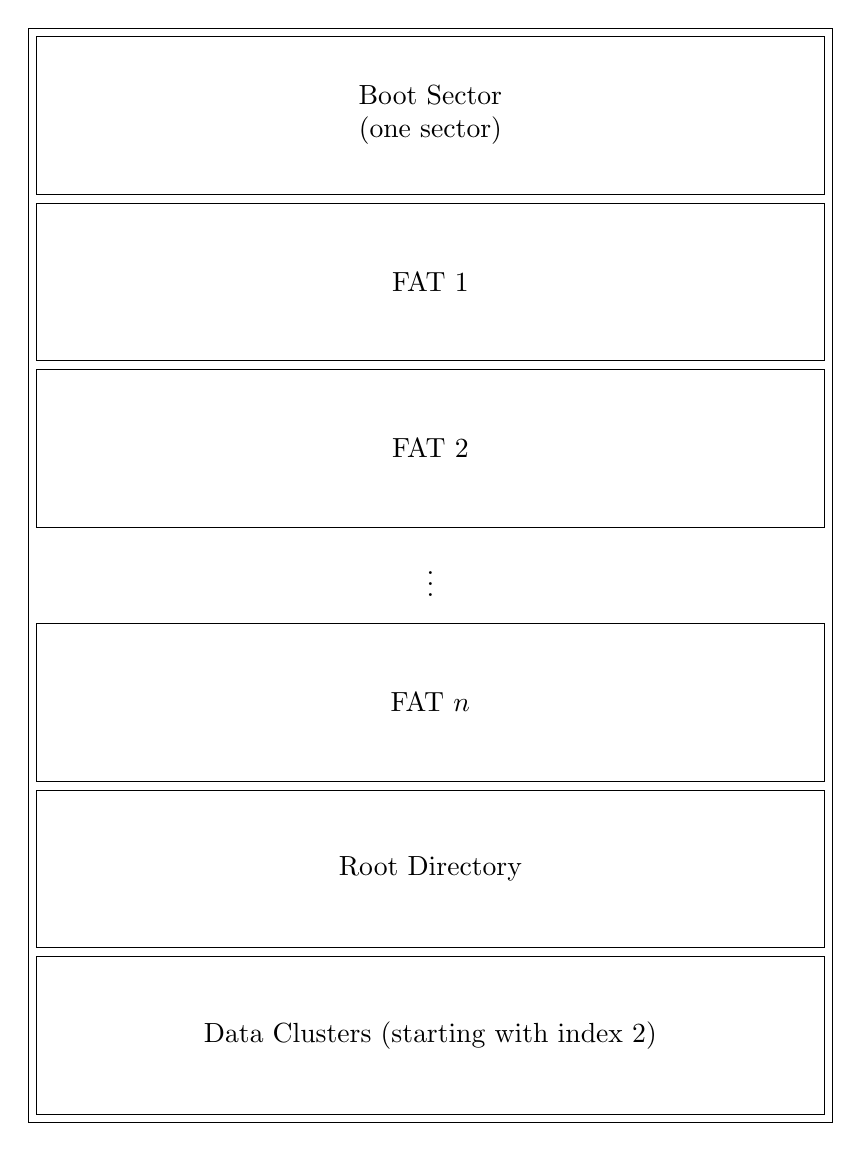
\begin{tikzpicture}
  \node[minimum width=10cm,minimum height=2cm,draw] (boot sector) at (0,0) {\parbox{8cm}{\centering Boot Sector \\ (one sector)}};
  \node[minimum width=10cm,minimum height=2cm,draw,anchor=north,yshift=-1mm] (fat 1) at (boot sector.south) {FAT 1};
  \node[minimum width=10cm,minimum height=2cm,draw,anchor=north,yshift=-1mm] (fat 2) at (fat 1.south) {FAT 2};
  \node[minimum width=10cm,minimum height=1cm,anchor=north,yshift=-1mm] (fat dots) at (fat 2.south) {\vdots};
  \node[minimum width=10cm,minimum height=2cm,draw,anchor=north,yshift=-1mm] (fat n) at (fat dots.south) {FAT $n$};
  \node[minimum width=10cm,minimum height=2cm,draw,anchor=north,yshift=-1mm] (root dir) at (fat n.south) {Root Directory};
  \node[minimum width=10cm,minimum height=2cm,draw,anchor=north,yshift=-1mm] (data) at (root dir.south) {Data Clusters (starting with index 2)};
  \draw ($ (boot sector.north west) + (-.1,.1) $) rectangle ($ (data.south east) + (.1,-.1) $);
\end{tikzpicture}


\end{document}